\chapter{Implementation}
In diesem Kapitel wird zun�chst die eingesetzte Entwicklungsumgebung und Programmiersprache vorgestellt.  


\section{Entwicklungsumgebung}
Als Entwicklungsumgebung f�r den Zustandsregler des Ballbots wird die ArduionoIDE eingesetzt, die in Abbildung \ref{fig:IDE} abgebildet ist. Die Hauptbestandteile dieser Entwicklungsumgebung umfasst einen Texteditor f�r das eigentliche Programm, eine Konsole f�r Fehler- und Kompilierungsmeldungen und einen seriellen Monitor f�r das Senden und Empfangen von Daten zwischen Computer und Board. Weiterhin eignet sich die Entwicklungsumgebung f�r den Einsatz, da ab der Version 1.6.4 diese �ber eine Bibliothek des eingesetzten OpenCR Board verf�gt. Allerdings ist diese Bibliothek nicht vorinstalliert, weshalb diese �ber den Boardverwalter nachinstalliert werden muss.[Git,Arduino]
\begin{figure}[htbp]
	\centering
		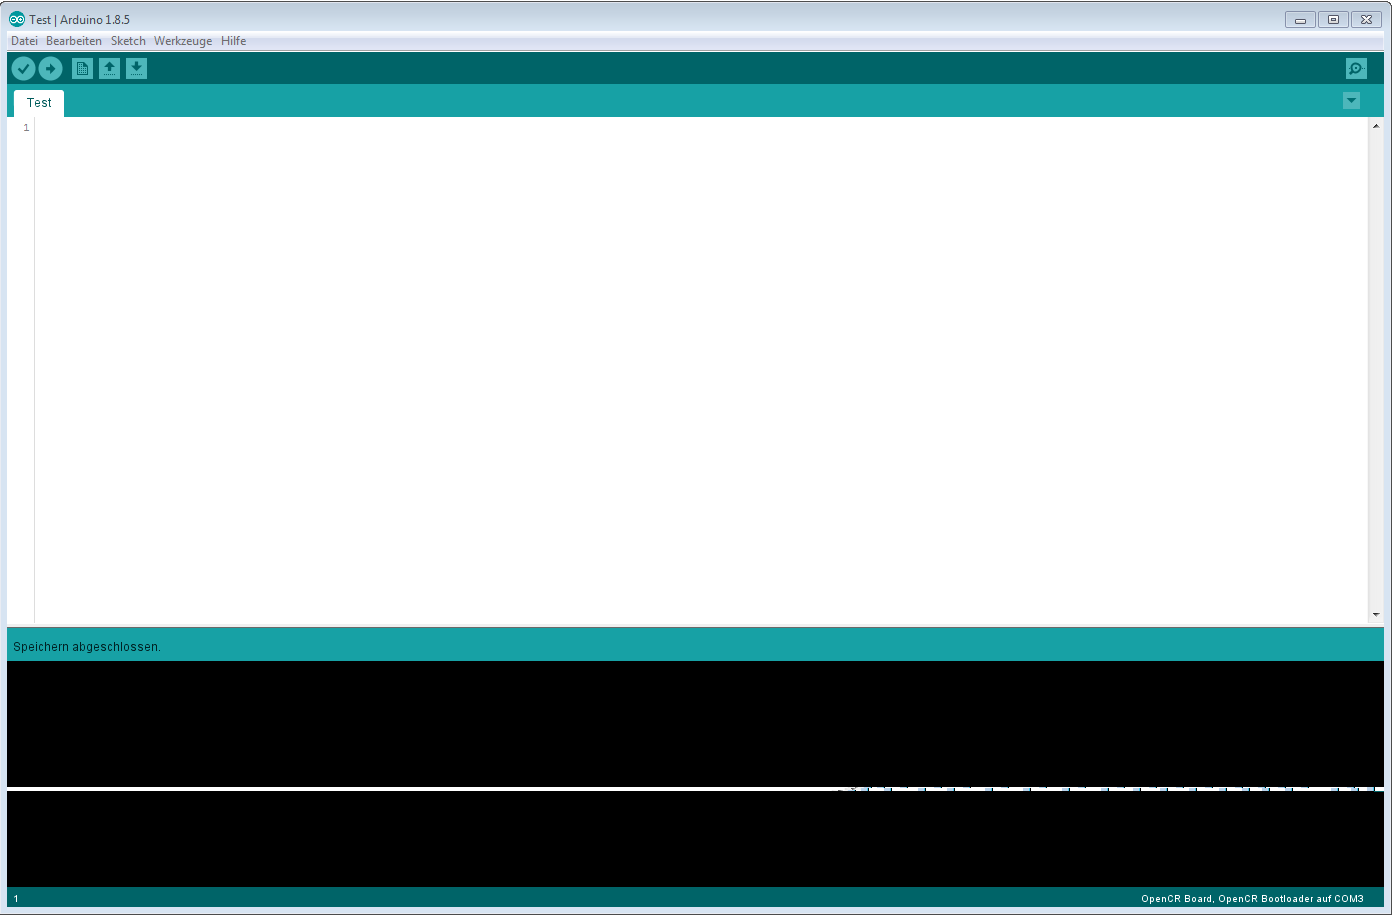
\includegraphics[width=0.70\textwidth]{Bilder/Florian/ArduinoIDE.PNG}
	\caption{Arduino Entwicklungsumgebung}
	\label{fig:IDE}
\end{figure}

Die Grundstruktur eines Programmes, die im Listing \ref{lst:Programm} dargestellt ist, gliedert sich in zwei Bereichen. In der Setup-Funktionen, die nur einmal beim Start des Board ausgef�hrt wird, werden verschieden Initialisierungen f�r den sp�teren Programmablauf festgelegt. Bei der Loop-Funktion handelt es sich um das eigentliche Programm, die als endlose Schleife durchlaufen wird. Werden f�r das Programm noch weitere Funktionen bzw. Variablen ben�tigt, m�ssen diese am Anfang oder am Ende eines Programmes definiert werden. 

\begin{lstlisting}[caption=Hier der Caption flo, label=lst:Programm, style = C_colored_smallfont]
void setup()	{
		// Diese Funktion wird nur beim Starten 
		// des entsprechen Boards einmal ausgef�hrt
}

void loop()	{
		// Diese Funktion in einer endlosen Schleife 
		// durchlaufen
}
\end{lstlisting}

Um die �bersichtlichkeit zu erh�hen, k�nnen Funktionen und Klassendefinitionen in seperate Dateien ausgelagert werden und im Hauptprogramm eingebunden werden. 


